\documentclass[10pt]{article}
\usepackage{spverbatim}
\usepackage{graphicx}
\usepackage{geometry}                % See geometry.pdf to learn the layout options. There are lots.
\geometry{letterpaper}                   % ... or a4paper or a5paper or ... 
%\geometry{landscape}                % Activate for for rotated page geometry
%\usepackage[parfill]{parskip}    % Activate to begin paragraphs with an empty line rather than an indent

%%%%%%%%%%%%%%%%%%%%
\newcommand{\hide}[1]{}

\usepackage{natbib}
\usepackage{xcolor}
\usepackage{url}
\usepackage{hyperref}
\usepackage{mathtools}

\hide{
\usepackage{amscd}
\usepackage{amsfonts}
\usepackage{amsmath}
\usepackage{amssymb}
\usepackage{amsthm}
\usepackage{cases}		 
\usepackage{cutwin}
\usepackage{enumerate}
\usepackage{epstopdf}
\usepackage{graphicx}
\usepackage{ifthen}
\usepackage{lipsum}
\usepackage{mathrsfs}	
\usepackage{multimedia}
\usepackage{wrapfig}
}
\bibliographystyle{humanbio}

	 
%\input{/usr/local/LATEX/Lee_newcommands.tex}
\newcommand{\itemlist}[1]{\begin{itemize}#1\end{itemize}}
\newcommand{\enumlist}[1]{\begin{enumerate}#1\end{enumerate}}
\newcommand{\desclist}[1]{\begin{description}#1\end{description}}

\newcommand{\Answer}[1]{\begin{quote}{\color{blue}#1}\end{quote}}
\newcommand{\AND}{\wedge}
\newcommand{\OR}{\vee}
\newcommand{\ra}{\rightarrow}
\newcommand{\lra}{\leftrightarrow}

\title {Advanced Artificial Inteligence Assignment }
\author{Grzegorz Sochacki \\}  

\begin{document}
\maketitle

\newpage

\tableofcontents{}

\newpage

\section{Tasks 1A and 1B}
These two tasks were approached by splitting the problem into two parts: Bayes Network Setup and Inference. The main reason for such a decision is due to availability of working code for inference algorithms from the workshop tutorials. Therefore, most of the code will treat setting up the networks for each task, while a brief discussion of inference algorithms will be added.

\subsection{Data structure}
Data structure provided in PriorSampling.py \citep{PriorSampling} was carried through the assignment, since code executing some of the algorithms was already developed during workshops. The difference is that these networks were placed in a separate class for code clarity as the number of networks has increased and additional code was needed to set up additional networks for assignments. "burglary" and "sprinkler" networks were kept for testing purposes. Networks are kept in an object of class "Network".

\subsection{Inference Algorithms}
It is important to notice that all algorithms have strengths and weaknesses, therefore the user has a choice to use one of three algorithms: Inference by Enumeration, Rejection Sampling and Weighted Likelihood. Moreover having more than one algorithm available gives a backup in case of a bug in code and allows for result comparison for ensuring the correctness of the result. Moreover, making "one fits all" is very hard due to the fact that probability distribution is learned from an external file, hence may differ between runs. Moreover, it should be noticed that comparing the execution time of the algorithms is quite useless, because of effects discussed in sections below. In some cases number of samples needed strongly depends on the network used, dataset, required precision, query variables and evidence. Such a comparison would be very specific and accurate only for the given set of variables listed.

\subsubsection{Inference by Enumeration}
This algorithm has a big advantage over other algorithms in terms of precision of the answer. While all of the algorithms are accurate, Enumeration is the only one in which precision is limited only by rounding errors. This is due to enumeration being an exact inference. Other algorithms' precision may be practically as high as Enumeration, but it depends on a number of samples. Moreover, precision function of other algorithms is dependent not only on a number of samples, but also on query and evidence. This makes the estimation of a number of samples needed very hard. 

The biggest disadvantage of Inference by Enumeration is the fact that some computations are performed more than once. This effect seems to be not significant for shallow networks and for queries with a large number of observations. In the first case it is because computed branches are short and additional computation does not take long. In the second case, high number of observations reduces a number of summations to be made, hence decreasing the overall number of branches to compute. This could be answered by employing Inference by Variable Elimination algorithm, but it is not a significant effect in the networks of size used for this assignment. \textbf{Therefore, this algorithm is a "go-to"algorithm for tasks 1A and 1B.}

\subsubsection{Inference by Rejection Sampling}
Inference by Rejection Sampling is the first of two inexact inference algorithms available in the program provided. It means that it is based on Monte Carlo sampling and needs multiple samples to produce an output. This algorithm is viewed as the worst of the three applied algorithms in terms of output precision. It rejects a lot of samples, therefore it will need the highest number of runs for a reliable answer. Moreover, the ratio of samples rejected is not constant. This ratio is equal to the probability that generated event happens to contain evidence values. For example, if a query about the "burglary" network contains "Earthquake = T" only 1 in 1000 of samples will pass. Therefore, this algorithm works best when evidence is a likely event. Other phenomena increasing the number of needed samples is that a reasonable number of samples both for query variable equal "True" and "False" must be collected. A quick example is having "Earthquake = True" as a query variable. After 1000 not rejected samples we should statistically have 999 "Earthquake = False" hits and 1 "Earthquake = True" hit. If the next sample comes out "Earthquake = True", it will almost double the computed probability of "Earthquake = True". It is hard to find a statistical solution to this problem, but a rule of thumb could be used to assess if enough samples have been collected. This could be based on computing standard deviation of probability distribution every bunch of samples and plotting it out. Once the standard deviation falls to a reasonable level and noise is reduced the output can be somewhat trusted.

The advantage of this algorithm is a simple implementation, therefore it can be trusted more than others from a safety point of view, due to less space for bugs.

\subsubsection{Inference by Weighted Likelihood}
Inference by Weighted Likelihood is essentially an improved version of Rejection Sampling. It does not reject samples, so the first bottleneck of Rejection Sampling is bypassed. Unfortunately, we still need a lot of hits to have any precision reliability. It is at the cost of added complexity.

\subsection{Task 1A: Network Setup}
Task 1A is a "rare disease problem", which can be represented as a two-node network, with a causal relationship between D(Disease) and test outcome (T). The structure is hardcoded inside the class Network. This network can then be filled with probabilities inputted by a user in the terminal. Three probabilities specified as input fully specify the network and class DiseaseNetworkSetup takes care of computing these probabilities and returning them in an array. The basic mechanism for this calculation is making use of the fact that the sum of probabilities of a complimentary event is equal to 1. While generating this network is a slight overhead it allows use of previously tested algorithms. Moreover, these algorithms were tested with bigger networks already, giving extra assurance of correct operation.

\subsection{Task 1A: User Manual}
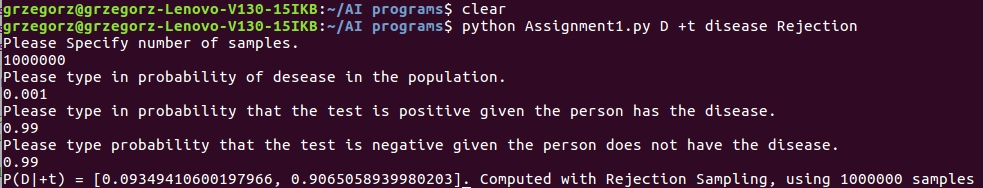
\includegraphics[width=\textwidth]{UserManual1.jpg}
The terminal screenshot attached above shows how to run the script for assignment 1A. Three arguments are needed to run the script correctly. These are: query variable as a capital letter, comma-separated evidence values and algorithm to be used. Evidence variables format is plus or minus and lower case letter. Possible values for the third argument are "Enumeration", "Rejection" and "Likelyhood". In the case above Task 1A was run using Rejection Sampling. Query variable was set to "D", evidence was set to "+t" and the network was set to disease. As Rejection Sampling was used, the script asks the user for a number of samples. Three questions for data specified in the task follows. The output is in a form of a normalized probability distribution, with first value corresponding to the query variable being true. 

\subsection{Task 1B: Network Setup}

This net was set up using the same structure as in task 1A and also has values of probabilities supplied by another class. In this case, this class is called SmokingNetworkSetup. For this task, learning probabilities is slightly harder than before and starts with reading in data from a csv file, which must be located in the same folder as a script and be called "assignmentDataset.csv". Each row is read into a separate array, which is essentially one event. Other function then counts the number of arrays that comply with values passed in the argument. From there formula provided in workshop week 3 \citep{Workshop3} is performed by another function. Using complementary events properties allows filling two spaces in the network data structure with one calculation.

\subsection{Task 1B: User Manual}
Using this network is very similar to running assignment 1A, just the name of the network and variable names need to be replaced. Reference the network structure in class Network to get exact variable names. An example of use is shown below. It asks for a probability of smoking given there was a car accident. This time Inference by Enumeration is used for presenting another algorithm.
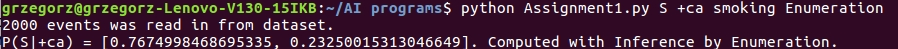
\includegraphics[width=\textwidth]{UserManual2.jpg}

\section{Task 2}
Task 2 was implemented with the use of a forward algorithm. The script is best run from a terminal and takes an observation sequence as an argument.

\subsection{Theoretical background}
According to \cite{bookA} probability of a given sequence occurring can be found in two ways. First of them is simple, but exponential time algorithm. It works by listing all possible hidden state combinations and computes a probability of each of them occurring. The next step is to multiply the probability of occurrence of each sequence by probability of producing a given sequence of observations. Finally, all these results are added to compute the final answer. This algorithm is not efficient and was not chosen for implementation. 

The goal can also be achieved with a p-complex forward algorithm\citep{bookA}. With each step, the algorithm based on current observation and the probability distribution of the previous hidden state computes a probability of getting that observation with each possible value of a hidden state. These values are not normalized, therefore each step returns the probability of observing the query sequence up to that observation. It should be noted that each sequence can happen for various hidden state sequences, therefore, probabilities of all trellis (in this case 2, due to 2 possible values of hidden state)need to be summed at the end. The exact formulas on which the algorithm is based can be found in lecture slides\citep{Lec7}.

\subsection{Implementation}
\begin{figure}[!h]
\caption{Graphical interpretation of forward algorithm \cite{bookA}.}
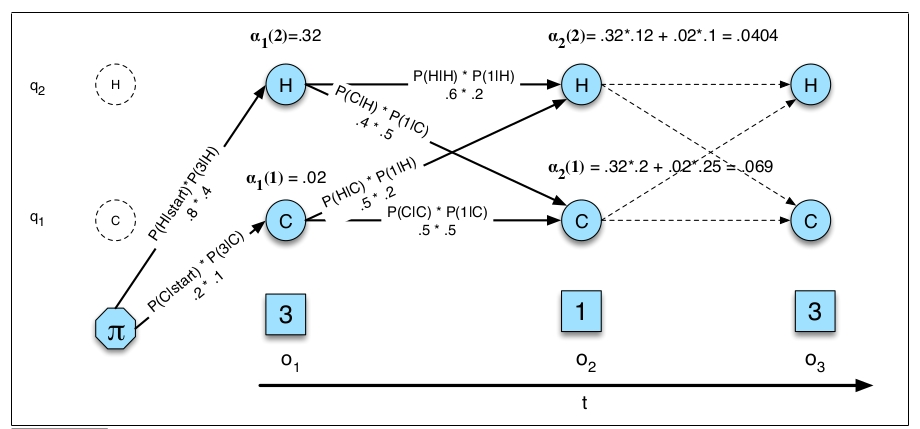
\includegraphics[width=\textwidth]{Trellis.jpg}
\end{figure}


The implementation is recursive in its nature, but was implemented as a for loop. Also, matrix notation suggested in Lecture 7 was not used\citep{Lec7.2}. The implementation sticks to an idea of progressing trellis step by step. The system time progression is best imagined by progression from left to right. The system can be then imagined as a row of three values - "ON" and "OFF" values of a hidden state and observation. Trellis form between each hidden state value at time t and t+1 at for all t. Trellis show hidden state transitions and are assigned a numerical value - the probability of a given state transition multiplied by the probability of resulting state producing a known observation. This value is then multiplied by the probability value of the state value of the trellis origin. At the resulting side of the trellis, both trellis values are summed. This value is usually denoted as $\alpha$. This system is graphically represented in a picture above. 
The software consists of two classes: Network and Hidden Markov. Class Network has hardcoded information about probability distributions in the network and provides methods for easy extraction of probability values. The Hidden Markov class contains arrays to store observations an $\alpha$ values, as well as forward algorithm execution. The number of steps if controlled by a for loop, based on input sequence length. The algorithm always uses last values of $\alpha$ stored, and adds new one by appending the storing matrix. This ensures the correct values are always used. Finally, method printProbability sums the values of both trellis, and prints the probability out.





\subsection{User Manual}

No additional files are needed to run the script and only one argument is required. The argument is a string of capital letters with no spaces and no commas. The string denotes a sequence of observations with time increasing from left to right. The observations are coded with a fist letter of their full name eg. "H" for "HOT". An example use for evaluating the probability of one-day long sequence is shown below.\newline
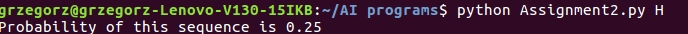
\includegraphics[width=\textwidth]{UserManual3.jpg}


\subsection{Results and Evaluation}
Firstly, the software was tested with a single observation input. This should give a mean of the probability of this observation in both hidden states. One of those tests output is shown in the section above. For all possible observations result was equal to on paper numerical solution. The sequence "CWHWC" returns a value shown below.\newline
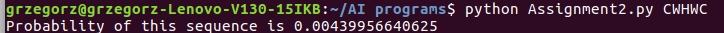
\includegraphics[width=\textwidth]{UserManual4.jpg}
\newline

While on paper calculations were not made for this specific sequence, a quick sanity check can be done. Both states "ON" and "OFF" states are equally probable, and will appear a similar amount of times in a long enough sequence. Also when the probability of each observation is averaged for both possible hidden states, the number is not far away from 1/3. Therefore, a rule of thumb is that the probability of a sequence of length n should be the same order of magnitude as 1/3 to the power of n, for reasonably small sequences. In this case, 0.00439 is the same order of magnitude to 0.0041. Therefore, the output looks reasonable.
\newpage

\bibliography{REF}


\newpage
\section{Appendix 1}
Appendix 1 contains a full code for script used to solve tasks 1A and 1B. It must be noticed that "spverbatim" was used to present the code, which splits long lines of code into few lines.


\begin{spverbatim}
import sys
import csv
import random

#This class is taking care about generating a network, which can be then fed into one of inference algorithms made during workshops. 
#Currently supported networks are: "burglary","sprinkler","disease","smoking", when latter two are for tasks 1A and 1B. 
#First two neteorks and the whole data structure are comming from PriorSampling.py provided on blackboard in week 5
class Network:
    CPTs={}

    def __init__(self, netID):
        self.initialiseNet(netID)		

    def initialiseNet(self, netID):
        if netID == "burglary":
            self.CPTs["B"]={"+b":0.001, "-b":0.999}
            self.CPTs["E"]={"+e":0.002, "-e":0.998}
            self.CPTs["A"]={"+a|+b+e":0.95, "-a|+b+e":0.05, 
					"+a|+b-e":0.94, "-a|+b-e":0.06,
					"+a|-b+e":0.29, "-a|-b+e":0.71,
					"+a|-b-e":0.001, "-a|-b-e":0.999}
            self.CPTs["J"]={"+j|+a":0.90, "-j|+a":0.10, 
					"+j|-a":0.05, "-j|-a":0.95}
            self.CPTs["M"]={"+m|+a":0.70, "-m|+a":0.30, 
					"+m|-a":0.01, "-m|-a":0.99}
            self.CPTs["order"]=["B", "E", "A", "J", "M"]
            self.CPTs["parents"]={"B":None, "E":None, "A":"B,E", "J":"A", "M":"A"}

        elif netID == "sprinkler":
            self.CPTs["C"]={"+c":0.50, "-c":0.50}
            self.CPTs["S"]={"+s|+c":0.10, "-s|+c":0.90, 
					"+s|-c":0.50, "-s|-c":0.50}
            self.CPTs["R"]={"+r|+c":0.80, "-r|+c":0.20, 
					"+r|-c":0.20, "-r|-c":0.80}
            self.CPTs["W"]={"+w|+s+r":0.99, "-w|+s+r":0.01, 
					"+w|+s-r":0.90, "-w|+s-r":0.10,
					"+w|-s+r":0.90, "-w|-s+r":0.10,
                    "+w|-s-r":0.00, "-w|-s-r":1.00}
            self.CPTs["order"]=["C", "S", "R", "W"]
            self.CPTs["parents"]={"C":None, "S":"C", "R":"C", "W":"S,R"}

        #setting network to "disease" triggers assignment 1A and will prompt user for information
        #Prompting the user and calculations are handled in class DiseaseNetworkSetup
        elif netID == "disease":
            #Prompting information and computing probailities
            networkGen = DiseaseNetworkSetup()
            [dT,  dF,  tTgT, tFgT, tTgF, tFgF] = networkGen.returnVariables(False)
            #Setting up actual network
            self.CPTs["D"] = {"+d":dT, "-d":dF}
            self.CPTs["T"] = {"+t|+d":tTgT, "-t|+d":tFgT, "+t|-d":tTgF,  "-t|-d":tFgF}
            self.CPTs["order"] = ["D",  "T"]
            self.CPTs["parents"] = {"D":None,  "T":"D"}
        
        #Setting network to smoking triggers code for Task 1B and could prompt user to give extra information depending on inpyt argumets
        #Actual copmputation of [robabilitis for the network will be handled by class SmokingNetworkSetup
        elif netID == "smoking":
            #Computing probabilities based on training data
            netGenerator = SmokingNetworkSetup()
            [aT, aF,  ppT, ppF, gT,  gF, bedT, bedF, alT, alF, sTgTT, sFgTT, sTgFT, sFgFT, sTgFF, sFgFF, sTgTF, sFgTF, yfTgT,  yfFgT, yfTgF, yfFgF, lcTgTT, lcFgTT, lcTgFT, lcFgFT, lcTgTF, lcFgTF, lcTgFF, lcFgFF, adTgT,  adFgT,  adTgF, adFgF, cTgTT, cFgTT, cTgFT, cFgFT, cTgFF, cFgFF, cTgTF, cFgTF, fTgTT, fFgTT, fTgFT, fFgFT, fTgFF, fFgFF, fTgTF, fFgTF, caTgTT, caFgTT, caTgFT, caFgFT, caTgFF, caFgFF, caTgTF, caFgTF] = netGenerator.generateProbabilities()
            #Actual network setup
            self.CPTs["A"] = {"+a":aT, "-a":aF}
            self.CPTs["PP"] = {"+pp":ppT, "-pp":ppF}
            self.CPTs["G"] = {"+g":gT, "-g":gF}
            self.CPTs["BED"] = {"+bed":bedT, "-bed":bedF}
            self.CPTs["AL"] = {"+al":alT, "-al":alF}
            self.CPTs["S"] = {"+s|+a+pp":sTgTT, "-s|+a+pp":sFgTT, "+s|-a+pp":sTgFT, "-s|-a+pp":sFgFT, "+s|-a-pp":sTgFF, "-s|-a-pp":sFgFF, "+s|+a-pp":sTgTF, "-s|+a-pp":sFgTF}
            self.CPTs["YF"] = {"+yf|+s":yfTgT,  "-yf|+s":yfFgT, "+yf|-s":yfTgF, "-yf|-s":yfFgF}
            self.CPTs["LC"] = {"+lc|+s+g":lcTgTT, "-lc|+s+g":lcFgTT, "+lc|-s+g":lcTgFT, "-lc|-s+g":lcFgFT, "+lc|+s-g":lcTgTF, "-lc|+s-g":lcFgTF, "+lc|-s-g":lcTgFF, "-lc|-s-g":lcFgFF}
            self.CPTs["AD"] = {"+ad|+g":adTgT,  "-ad|+g":adFgT,  "+ad|-g":adTgF, "-ad|-g":adFgF}
            self.CPTs["C"] = {"+c|+al+lc":cTgTT, "-c|+al+lc":cFgTT, "+c|-al+lc":cTgFT, "-c|-al+lc":cFgFT, "+c|-al-lc":cTgFF, "-c|-al-lc":cFgFF, "+c|+al-lc":cTgTF, "-c|+al-lc":cFgTF}
            self.CPTs["F"] = {"+f|+lc+c":fTgTT, "-f|+lc+c":fFgTT, "+f|-lc+c":fTgFT, "-f|-lc+c":fFgFT, "+f|-lc-c":fTgFF, "-f|-lc-c":fFgFF, "+f|+lc-c":fTgTF, "-f|+lc-c":fFgTF}
            self.CPTs["CA"] = {"+ca|+ad+f":caTgTT, "-ca|+ad+f":caFgTT, "+ca|-ad+f":caTgFT, "-ca|-ad+f":caFgFT, "+ca|-ad-f":caTgFF, "-ca|-ad-f":caFgFF, "+ca|+ad-f":caTgTF, "-ca|+ad-f":caFgTF}
            self.CPTs["order"] = ["A", "PP", "G", "BED", "AL", "S", "YF", "LC", "AD", "C", "F", "CA"]
            self.CPTs["parents"] = {"A":None, "PP":None, "G":None, "BED":None, "AL":None, "S":"A,PP", "YF":"S", "LC":"S,G", "AD":"G", "C":"AL,LC", "F":"LC,C", "CA":"AD,F"}
            
        #Error message in case of typo in the network name
        else:
            print("UNKNOWN network="+str(netID))
            exit(0)

#This class sets up a disease network for task 1A, It asks user for probabilities specified in the brief and computes rest of probabilities needed to specify a network
#Basic rule used here it the fact that probabilities notA|Evidence and A|Evidence must add up to 1
class DiseaseNetworkSetup:
    dT = 0.0
    dF = 0.0
    tTgT = 0.0
    tFgT = 0.0
    tFgT = 0.0
    tFgF = 0.0
    
    def __init__(self):
        #Prompting for probability of desease
        print("Please type in probability of desease in the population.")
        self.dT = input()
        self.dF = 1.0 - self.dT
        #First prompt for quality of the test
        print("Please type in probability that the test is positive given the person has the disease.")
        self.tTgT = input()
        self.tFgT = 1 - self.tTgT
        print("Please type probability that the test is negative given the person does not have the disease.")
        self.tFgF = input()
        self.tTgF = 1 - self.tFgF
    
    #this functions returns variables stored in the object, with an option to print them out for debuggin purpose
    def returnVariables(self,  ifPrint):
        if ifPrint == True:
            print([self.dT,  self.dF,  self.tTgT, self.tFgT, self.tTgF, self.tFgF])
        return [self.dT,  self.dF,  self.tTgT, self.tFgT, self.tTgF, self.tFgF]


#This class takes care of computing conditional probabilities for "smoking" network
#data is read from a file called assignmentDataset.csv located in the same file as the script
#Calculation is made using the algorithm presented in workshop materials.
class SmokingNetworkSetup:
    #Preprogrammed order for the variables IN CSV NOT NETWORK
    order_in_csv = ["S",  "YF",  "A",  "PP",  "G",  "AD",  "BED",  "CA",  "F",  "AL",  "C", "LC"]
    events = []
    purged_events = []
    #Init, taking care of reading the file, events are being stored as an array of 1s and 0s in array events
    def __init__(self):
        #CSV reading
        with open('assignmentDataset.csv') as csv_file:
            csv_reader = csv.reader(csv_file, delimiter=',')
            row_count = 0
            #converting all rows exept first into events
            for row in csv_reader:
                if row_count != 0:
                    self.events.append(row)
                    #print(self.events[row_count-1])
                    row_count += 1
                else:
                    row_count += 1
        print(str(row_count-1) + " events was read in from dataset.")

    #This function returns an array containing all probabilities needed to fully specify smoking network
    def generateProbabilities(self):
        #generate probabilities for node A
        [aT,  aF] = self.probabilityDistribution("+a", "")
        #generate probabilities for node PP
        [ppT,  ppF] = self.probabilityDistribution("+pp", "")
        #generate probabilities for node G
        [gT,  gF] = self.probabilityDistribution("+g", "")
        #generate probabilities for node BED
        [bedT,  bedF] = self.probabilityDistribution("+bed", "")
        #generate probabilities for node AL
        [alT,  alF] = self.probabilityDistribution("+al", "")
        #generate probabilities for node S (Smoking)
        [sTgTT, sFgTT] = self.probabilityDistribution("+s", "+a,+pp")
        [sTgFT, sFgFT] = self.probabilityDistribution("+s", "-a,+pp")
        [sTgFF, sFgFF] = self.probabilityDistribution("+s", "-a,-pp")
        [sTgTF, sFgTF] = self.probabilityDistribution("+s", "+a,-pp")
        #generate probabilities for node YF (Yellow Fingers)
        [yfTgT, yfFgT] = self.probabilityDistribution("+yf", "+s")
        [yfTgF, yfFgF] = self.probabilityDistribution("+yf", "-s")
        #generate probabilities for node LC (Lung Cancer)
        [lcTgTT, lcFgTT] = self.probabilityDistribution("+lc", "+s,+g")
        [lcTgFT, lcFgFT] = self.probabilityDistribution("+lc", "-s,+g")
        [lcTgFF, lcFgFF] = self.probabilityDistribution("+lc", "-s,-g")
        [lcTgTF, lcFgTF] = self.probabilityDistribution("+lc", "+s,-g")
        #generate probabilities for node AD (AttentionDisorder)
        [adTgT, adFgT] = self.probabilityDistribution("+ad", "+g")
        [adTgF, adFgF] = self.probabilityDistribution("+ad", "+g")
        #generate probabilities for node C (caughing)
        [cTgTT, cFgTT] = self.probabilityDistribution("+c", "+al,+lc")
        [cTgFT, cFgFT] = self.probabilityDistribution("+c", "-al,+lc")
        [cTgFF, cFgFF] = self.probabilityDistribution("+c", "-al,-lc")
        [cTgTF, cFgTF] = self.probabilityDistribution("+c", "+al,-lc")
        #generate probabilities for node F (fatigue)
        [fTgTT, fFgTT] = self.probabilityDistribution("+f", "+c,+lc")
        [fTgFT, fFgFT] = self.probabilityDistribution("+f", "-c,+lc")
        [fTgFF, fFgFF] = self.probabilityDistribution("+f", "-c,-lc")
        [fTgTF, fFgTF] = self.probabilityDistribution("+f", "-c,-lc")
        #generate probabilities for node CA (Car Accident)
        [caTgTT, caFgTT] = self.probabilityDistribution("+ca", "+ad,+f")
        [caTgFT, caFgFT] = self.probabilityDistribution("+ca", "-ad,+f")
        [caTgFF, caFgFF] = self.probabilityDistribution("+ca", "-ad,-f")
        [caTgTF, caFgTF] = self.probabilityDistribution("+ca", "+ad,-f")
        
        
        return [aT, aF,  ppT, ppF, gT,  gF, bedT, bedF, alT, alF, sTgTT, sFgTT, sTgFT, sFgFT, sTgFF, sFgFF, sTgTF, sFgTF, yfTgT,  yfFgT, yfTgF, yfFgF, lcTgTT, lcFgTT, lcTgFT, lcFgFT, lcTgTF, lcFgTF, lcTgFF, lcFgFF, adTgT,  adFgT,  adTgF, adFgF, cTgTT, cFgTT, cTgFT, cFgFT, cTgFF, cFgFF, cTgTF, cFgTF, fTgTT, fFgTT, fTgFT, fFgFT, fTgFF, fFgFF, fTgTF, fFgTF, caTgTT, caFgTT, caTgFT, caFgFT, caTgFF, caFgFF, caTgTF, caFgTF]
    
    #This function conputes conditional probability that distribution of variable given evidence
    #The convention for output is [P(true)|evidence, P(false)|evidence]
    def probabilityDistribution(self, variable, evidence):
        pT = (self.countEvents(evidence+","+variable)+1)/(self.countEvents(evidence) + 2)
        return [pT,  1-pT]
        
    #This function preselects events so only those meeting the observation remain
    #format here is like +b,+m (for input)
    def countEvents(self, conditions):
        events_count = 0
        fail = 0
        #clean the purged events variable
        self.purged_events = []
        for e in self.events:
            #reset fail flag
            fail = 0
            #do chceck only if conditions actually exist
            #print("Conditions are:" + conditions + ".")
            if len(conditions) != 0:
                for c in conditions.split(","):
                    #do this only when c is not None, this happens when computing nodes without parents
                    if len(c) != 0:
                        #was the condition 1 or 0?
                        value = 4
                        if "+" in c:
                            value = 1
                        if "-" in c:
                            value = 0
                        #drop + or - from the variable
                        c = c[1:len(c)]
                        #Get index in order of csv
                        c = c.upper()
                        #print(c)
                        index = self.getIndexCSV(c)
                        if int(e[index]) != int(value):
                            #this condition was not met, set the fail flag
                            fail = 1
            #copy event to purged_events
            if fail == 0:
                events_count += 1
        #print(str(events_count) + " events met conditions: " + conditions)
        return float(events_count)
    
    #This function returns index of the variable in csv order, effectively telling how which column to read for given variable
    def getIndexCSV(self, var):
        counter = 0
        for c in self.order_in_csv:
            if var == self.order_in_csv[counter]:
                return counter
            counter += 1


#This class is performs all tasks neede to go from reading in network to answering a query
#Algorithm used is Rejection Sampling
#Some of code for thi class (making a smaple) is comming form PriorSampling.py provided in workshop materials
class RejectionSampling:
    #These are class variables, shared among all objects
    #variable for holding a prior sampling class's object
    net = None
    #Counter for samples where query Variable is true(after rejecting inconsistent samples)
    positive_outcomes = 0
    #otherwise counter
    negative_outcomes = 0
    
    def __init__(self, bn):
        #read in a network
        self.net=Network(bn)
    
    #This function samples a single variable knowing probability distribution
    #it produces a random numbe 0 to 1 and compares it to the probability
    def sampleVariable(self, CPT, conditional):
        sampledValue=None
        randnumber=random.random()

        value1=CPT["+"+conditional]
        #value2=CPT["-"+conditional]

        if randnumber<=value1:
            sampledValue="+"+conditional
        else:
            sampledValue="-"+conditional

        return sampledValue.split("|")[0]
    
    #This function runs the sampleing function over all variables in odrd specified in order, so parents are alwyas sampled before childrens.
    def sampleVariables(self, printEvent):
        event=[]
        sampledVars={}

        for variable in self.net.CPTs["order"]:
            evidence=""
            conditional=""
            parents=self.net.CPTs["parents"][variable]
            if parents==None:
                conditional=variable.lower()
            else:
                for parent in parents.split(","):
                    evidence+=sampledVars[parent]
                conditional=variable.lower()+"|"+evidence

            sampledValue=self.sampleVariable(self.net.CPTs[variable], conditional)
            event.append(sampledValue)
            sampledVars[variable]=sampledValue
				
        if printEvent: print(event)
        return event
    
    #this function is to return true if the sample of network is consistent with evidence
    #basically checks if values of evidence variables are same in query and sample
    def isConsistentWithEvidence(self,  evidence,  event):
        #If there is no evidence to consider
        if evidence == "": 
            return True
     
        #This splits the string in strings at "," character
        for i in evidence.split(","):
            #if that string is not in event sampled, return false
            if i not in event:
                return False
                
        #If all tests passsed, return true
	#print("Consistent!")
        return True
    
    def getIndexOfVariableInEventList(self,  queryVariable):
        #Load order from the net definition
        variables = self.net.CPTs["order"]
        #Look for the query variable in the order list
        for i in range(0,  len(variables)):
            if variables[i] == queryVariable:
                return i 
        
        #No idea why?
        return None
                
    
    #This function gets a single sample of the whole network , rejects if not consistence with evidence, 
    #otherwise adjust appropriet counter to get ammout of samples where query variable was true and false
    def singleEventGenerationAndEvaluation(self, evidence,  X):
        #This samples the network  and creates the event
        event = self.sampleVariables(False)
        #proceed only when event is consistant with evidence otherwise sample is being rejected
        if self.isConsistentWithEvidence(evidence,  event):
            #Now its time to figure out if query variable is true or false in given sample
            #first find the index of the variable in event passed from prior sampling
            index = self.getIndexOfVariableInEventList(X)
            if ('+' in event[index]):
                self.positive_outcomes +=1
            else:
                self.negative_outcomes +=1
           
    #This function repeats the treatment of a single sample numberOfSamples times
    def eventLoop(self,  numberOfSamples, evidence,  X):
        for i in range(1,  numberOfSamples):
            self.singleEventGenerationAndEvaluation(evidence,  X)
    
    #Normalizes probability distribution
    def normalize(self):
        #sum of all not rejected events
        sum =float( self.negative_outcomes + self.positive_outcomes)
        distibution = [float(self.positive_outcomes)/sum, float(self.negative_outcomes)/sum]
        return distibution
        
    #Printout of the probability istribution
    def printProbabilityDistribution(self, numberOfSamples,  evidence,  X):
        #runs the dampling and evaluation
        self.eventLoop(numberOfSamples,  evidence,  X)
        distribution = self.normalize()
        print("P("+X+"|"+evidence+") = " + str(distribution)+". Computed with Rejection Sampling, using " + str(numberOfSamples) + " samples"), 
        #print(distribution)
        

#This class is performs all tasks neede to go from reading in network to answering a query
#Algorithm used is Inference by Enumeration
class Enumeration:
    #Variable to store network to work on.
    net = None
    
    def __init__(self,  bn):
        self.net = Network(bn)
        
    #this function takes unnormalized probability distribution and prints out a normalized probability distribution    
    def printProbabilityDistribution(self, evidence, X):
        #get unnormalized probability distribution
        unnormalized_distribution = self.getNotNormalizedProbabilities(evidence,  X)
        #normalize
        sum = unnormalized_distribution[0] + unnormalized_distribution[1]
        normalized_distribution = [0, 0]
        normalized_distribution[0] = unnormalized_distribution[0]/sum
        normalized_distribution[1] = unnormalized_distribution[1]/sum
        print("P("+X+"|"+evidence+") = " + str(normalized_distribution)+". Computed with Inference by Enumeration.")
    
    #This function computes probability for query variable to be true and false, these are not normalized yet
    def getNotNormalizedProbabilities(self,  evidence,  X):
        #Load variables from network
        variablesToEnumerate = self.net.CPTs["order"]
        #Extending evidence with the True and False versions of query variable
        ext_evidenceT = evidence + ",+" + X.lower()
        ext_evidenceF = evidence + ",-" + X.lower()
        ProbT = self.enumerate(variablesToEnumerate, ext_evidenceT)
        ProbF = self.enumerate(variablesToEnumerate, ext_evidenceF)
        return [ProbT,  ProbF]
    
    #This function uses inference by enumeration to compute a probability of an event specified in extended evidence to be true.
    def enumerate(self, variables,  extended_evidence):
        # That is the end of recursion, effectively multiplies the value from previous iteration by 1
        if len(variables) == 0:
            #print("NO VARIABLES LEFT")
            return 1.0
        #Take next variable and prepare true and false strings which can be queried
        Y = variables[0]
        y = Y.lower()
        yT = "+" + y
        yF = "-" + y
        #Check if that variable is in evidence string
        if yT in extended_evidence.split(",") or yF in extended_evidence.split(","):
            #if it is the value can be plugged from the network dictionary
            return self.net.CPTs[Y][self.conditionalString(Y, extended_evidence,  False)] * self.enumerate(variables[1:len(variables)], extended_evidence)
        else:
            #Otherwise reutrn sum of both options, when the variable is tru or false
            sum1 = self.net.CPTs[Y]["+" + y + self.conditionalString(Y, extended_evidence + ",+" + y,  True)] * self.enumerate(variables[1:len(variables)], extended_evidence + ",+" + y)
            sum2 = self.net.CPTs[Y]["-" + y + self.conditionalString(Y, extended_evidence + ",-" + y,  True)] * self.enumerate(variables[1:len(variables)], extended_evidence + ",-" + y)
            return sum1 + sum2
    
    #This is a helpful function which constructs a key strings, which can be used accesing values in CPTs
    def conditionalString(self, Y, evidence,  partial):
        string = ""
        #do not run this if only partial string is needed (when arbitrary setting the dependent variable when summing)
        if partial == False:
            #first part of string
            string = self.valueInEvidence(Y, evidence)
        #if there is no parents, exit here
        if self.net.CPTs["parents"][Y] == None:
            return string
        string += "|"
        #print("Parents: " + self.net.CPTs["parents"][Y])
        for b in self.net.CPTs["parents"][Y].split(","):
            #print("Parent loop in conditional string generation")
            string += self.valueInEvidence(b,  evidence)
            #print("Updated string in parents loop: " + string)
        #print(string)
        return string
        
    #Function to get value of single variable from the whole evidence string
    def valueInEvidence(self, Y, evidence):
        output_string = ""
        y = Y.lower()
        if ("+"+ y) in evidence.split(","):
            output_string = "+" + y
        if ("-"+ y) in evidence.split(","):
            output_string = "-" + y
        #print("value of evidence output string" + output_string)
        return output_string


#This class is performs all tasks neede to go from reading in network to answering a query
#Algorithm used is Weighted Likelyhood
class WeightedLikelyhood:
    #These are class variables, shared among all objects
    #variable for holding a prior sampling class's object
    net = None
    #Counter for samples where query Variable is true(after rejecting inconsistent samples)
    positive_outcomes = 0.0
    #otherwise counter
    negative_outcomes = 0.0
    
    #Read in the network
    def __init__(self, bn):
        #create object from sampling class
        self.net = Network(bn)
    
    #creates a single sample of thenetwork
    def oneWeightedSample(self,  e,  X):
        event = []
        w = 1
        #Run a loop and either sample or change a weigth
        for i in self.net.CPTs["order"]:
            #print(event)
            #Check if the variable is in evidence string
            #n = self.getIndexOfVariableInEventList(i)
            if i.lower() in e:
                #get value of variable from evidence
                bool = self.trueOrFalse(i,  e)
                #set this value to the event
                event.append(bool)
                #adjust weight accordingly
                w = w * self.returnVariableProbability(bool,  i,  event)
            else:
                #sample the variable from conditional probability and add to event
                logicValue = self.sample(self.returnVariableProbability(True, i,  event))
                event.append(logicValue)
        #Is the value of query variable true in the event?
        queryBool = self.isQueryTrue(X,  event)
        return [event,  w, queryBool]
    
    def isQueryTrue(self, X,  event):
        #get index of query variable in the event array
        index = self.getIndexOfVariableInEventList(X)
        return event[index]
    
    #functions checks if the variable in the event was true or false
    def trueOrFalse(self,  variable,  e):
        trueString = "+"+variable.lower()
        falseString = "-"+variable.lower()
        if trueString in e:
            return True
        if falseString in e:
            return False
        return None
    
    #This function knowing event part sampled so far gets a chance that the variable is bool
    def returnVariableProbability(self, bool,  var, event):
        varLower = var.lower()
        #if variable has no parents, return nonconditional probability
        parents=self.net.CPTs["parents"][var]
        if parents == None:
            #print("No Parents")
            return self.net.CPTs[var]["+"+varLower]
        
        #if has parents fetch value of parents from event so far and get conditional probability
        askString = "+"+varLower+"|"
        #run loop for all parents
        for parent in parents.split(","):
            #print(parent)
            #get index in event matrix for this parent
            n = self.getIndexOfVariableInEventList(parent)
            #print(n)
            #modify ask string depending on the current event true/false values
            if event[n] == True:
                askString = askString + "+"+parent.lower()
            else:
                askString = askString +"-"+parent.lower()
        
        #return the conditional probablity based on the knowledge from before the sample
        if bool == True:
            return self.net.CPTs[var][askString]
        else:
            return 1 - self.net.CPTs[var][askString]
     
  
    
    def getIndexOfVariableInEventList(self,  queryVariable):
        #Load order from the net definition
        variables = self.net.CPTs["order"]
        #Look for the query variable in the order list
        for i in range(0,  len(variables)):
            #print(i)
            if variables[i] == queryVariable:
                return i 
    
    #This function takes probability that event is true and returns TRue or False
    def sample(self, prob):
        #get random number
        randnumber=random.random()
        if randnumber > prob:
            return False
        else:
            return True
    
    #This function repeats the creation of an event with weight and assigns weights to positive_outcomes and negative outcomes
    def eventLoop(self,  numberOfSamples, evidence,  X):
        for i in range(1,  numberOfSamples):
            #generate event
            weightedSample = self.oneWeightedSample(evidence, X)
            #print(weightedSample)
            #add weight as a positive or negative outcome
            if weightedSample[2] == True:
                self.positive_outcomes += weightedSample[1]
            if weightedSample[2] == False:
                self.negative_outcomes += weightedSample[1]
    
    #Returns a normalized probability distribution
    def normalize(self):
        #sum of all not rejected events
        sum = float( self.negative_outcomes + self.positive_outcomes)
        distibution = [float(self.positive_outcomes)/sum, float(self.negative_outcomes)/sum]
        return distibution
        

    def printProbabilityDistribution(self, numberOfSamples,  evidence,  X):
        #runs the dampling and evaluation
        self.eventLoop(numberOfSamples,  evidence,  X)
        distribution = self.normalize()
        print("P("+X+"|"+evidence+") = " + str(distribution) + ". It was computed using Weighted Likelyhood with " + numberOfSamples + " samples.")



if __name__ == "__main__":
    #X is the query variable, for example for Burglray net use one of B E A J M
    X = str(sys.argv[1])
    #evidence observed, they are treated as a known information, so for example b=1, c=1, b=0 and c=1
    #these would be inputed as +b, +c, -b,+c
    evidence = str(sys.argv[2])
    #bn is a bayes network used by sampling class prior sampling
    #possible values are "burglary", "sprinkler", "disease" , "smoking"
    bn = str(sys.argv[3])
    #Choose which inference algorithm is to be used
    #Possible values are Enumeration, Rejection and Likelyhood
    infAlg = str(sys.argv[4])
    
    #Decision of which class to initializ and use for computation
    if infAlg == "Enumeration":
        IbE = Enumeration(bn)
        IbE.printProbabilityDistribution(evidence,  X)
    elif infAlg == "Rejection":
        print("Please Specify number of samples.")
        N = input()
        RJ = RejectionSampling(bn)
        RJ.printProbabilityDistribution(N,  evidence,  X)
    elif infAlg == "Likelyhood":
        print("Please Specify number of samples.")
        N = input()
        WL = WeightedLikelyhood(bn)
        WL.printProbabilityDistribution(N, evidence,  X)
    else:
        print("Invalid algorithm type.")
        
\end{spverbatim}



\newpage
\section{Appendix 2}
Appendix 2 contains a full code for script used to solve task 2 of the assignment. It must be noticed that "spverbatim" was used to present the code, which splits long lines of code into few lines.


\begin{spverbatim}



import sys

#This class stores a network and provides method to return probability values from this network
class Network:
    CPTs={}

    def __init__(self, netID):
        self.networkSetup(netID)		

    def networkSetup(self, netID):
        
        if netID == "weather":
            #Hidden States Transitions, convention is that CPTs[ON][OFF] is probability of ON given last time step it was OFF
            self.CPTs["ON"]={"ON":0.7, "OFF":0.3}
            self.CPTs["OFF"]={"ON":0.3, "OFF":0.7}
            #Conditional probabilities of observing observable variables given the hidden state
            self.CPTs["HOT"]={"ON":0.4, "OFF":0.1}
            self.CPTs["WARM"]={"ON":0.4, "OFF":0.45}
            self.CPTs["COLD"]={"ON":0.2, "OFF":0.45}
        else:
            print("UNKNOWN network="+str(netID))
            exit(0)

    #returning a transition probability between two hidden states
    def returnHiddenProbability(self, now,  before):
        return self.CPTs[now][before]
    
    #returns probability of a given observation based on current hidden state
    def returnObservationProbability(self, observation,  hiddenState):
        return self.CPTs[observation][hiddenState]
        
#This class performs forward algorithm and prints out probability 
#of appearance of the query obseravation 
class HiddenMarkow:
    net = None
    observations = []
    alphaON = [0.5] 
    alphaOFF = [0.5]
    
    def __init__(self, inputString):
        #Read in network information
        self.net = Network("weather")
        self.observations = [x for x in inputString]
        #go from single letter to full words for observations
        #This is to allow the user to use single letters for faster chanes of queries
        for i in range(0,  len(self.observations)):
            if self.observations[i] == "H":
                self.observations[i] = "HOT"
                
            if self.observations[i] == "C":
                self.observations[i] = "COLD"
            if self.observations[i] == "W":
                self.observations[i] = "WARM"
        for i in range(0,  len(self.observations)):
            self.forward(self.observations[i])
        #print(self.alphaON)
        #print(self.alphaOFF)
        self.printProbability()
     
    #Runs the forword algorithm without normalization
    #Weights of trellis are stored in self.alphaON/OFF by appending these arrays
    def forward(self, observationToday):
        previousAlphaON = self.alphaON[len(self.alphaON) - 1]
        previousAlphaOFF = self.alphaOFF[len(self.alphaOFF) - 1]
        #For taday being ON
        alphaON = self.net.returnObservationProbability(observationToday, "ON") * (self.net.returnHiddenProbability("ON", "ON") * previousAlphaON + self.net.returnHiddenProbability("ON", "OFF") * previousAlphaOFF)
        #for today being OFF
        alphaOFF = self.net.returnObservationProbability(observationToday, "OFF") * (self.net.returnHiddenProbability("OFF", "ON") * previousAlphaON + self.net.returnHiddenProbability("OFF", "OFF") * previousAlphaOFF)
        self.alphaON.append(alphaON)
        self.alphaOFF.append(alphaOFF)

    #Computes probability by adding weights of both trellis
    def printProbability(self):
        prob = self.alphaON[len(self.alphaON) - 1] + self.alphaOFF[len(self.alphaOFF) - 1]
        print("Probability of this sequence is " + str(prob))

#Code run on the start of the script
if __name__ == "__main__":
    #Input string containing the observation string in form like CHWHC
    inputString = str(sys.argv[1])
    HM = HiddenMarkow(inputString)


\end{spverbatim}
\end{document}




